\documentclass[]{sig}
\usepackage{graphicx}
\usepackage{mathtools}
\usepackage{amsmath}
\usepackage[utf8]{inputenc}
\usepackage{cleveref}
\usepackage{listings}
\usepackage{array}
\usepackage{breqn}
\usepackage{tikz}
\usetikzlibrary{automata,positioning}
\newtheorem{mydef}{Definition}
\lstset{
	basicstyle=\itshape,
	xleftmargin=2em,
	literate={->}{$\rightarrow$}{2}
	{α}{$\alpha$}{1}
	{δ}{$\delta$}{1}
}
\crefname{section}{§}{§§}
\Crefname{section}{§}{§§}

\usepackage{float}
%opening
\title{Genesis : End-to-End Policy Enforcement by Switch Table Synthesis }
\author{Kausik Subramanian \\
	University of Wisconsin-Madison}

\begin{document}

\maketitle

\begin{abstract}
Operators in enterprise and datacenter networks deal with complex end-to-end policies for a large number of classes like reachabilities, middlebox traversals and isolation policies, and dealing with these policies separately and enforcing them at switch-level rules is cumbersome. To tackle this, we create a tool Genesis which supports a rich suite of end-to-end policies which the network operator can specify using a high-level API. Genesis converts the policy enforcement problem to a SMT instance and synthesizes switch rules using a SMT solver (Z3) which can be used by a controller to deploy to the topology.
\end{abstract}

\section{Introduction}
%[Intro] 
Network operators of enterprise and cloud datacenter networks deal with hundreds of switches and thousands of traffic classes desiring diverse end-to-end policies. However, in real-life, the process of policy enforcement by network operators is manual and ad-hoc, leading to mis-configurations which have severe performance and security impacts. With the boom in cloud services, datacenter networks deal with thousands of packet classes which are not constant, but in flux, thus, making it difficult to enforce them manually. 

The bare minimum need is \emph{reachability} for hosts from ingress to egress switches in these networks. 
%[Middlebox]
 With the recent advent of complex packet processing middleboxes like like intrusion detection systems, firewalls, load balancers etc, a feature of use is to specify the middleboxes a particular flow would like to traverse. 

%[Isolation] 
With the advent of multi-tenant cloud services, a desired feature cloud providers need to support is various Quality of Service guarantees. The current Service Level Agreements (SLA) provided are centered around compute, storage, or Internet traffic. The lack of a good network management system, there exists no provisions for providing SLAs in terms of network performance guarantees among the VMs. Lack of network guarantees leads to unpredictability of performance for distributed applications. Tenants may have to run VMs for a longer time, because the network turns out to be a bottleneck. This leads to increased expense for tenants. Also, multi-tenant clouds are susceptible to network attacks. For example, if two tenants share a link in the datacenter, one tenant could hog the bandwidth on the link, and the other tenant would suffer due to unequal distribution of bandwidth. To combat this, cloud operators rate-limit the VMs, but this can reduce link utilization as tenants may not be using the complete share of their bandwidth. An approach to remove interference between tenant flows is to ensure the tenant flows do not share links in the datacenter, and recent datacenter topologies like fat-trees provides multiple paths from one layer to another and thus, we can route different tenants through different paths. Thus, support for link isolation policies is a very important feature for cloud operators. 

There has been a lot of work in the field of policy enforcement in networks, like bandwidth provisioning in Merlin \cite{Merlin}, and middlebox policy enforcement in SIMPLE \cite{simple}. However, the approach followed in these works are catered to the specific policies, and thus, difficult to extend it to, for example, provide isolation of paths. An ideal policy enforcement system for network operators would support complex and diverse policies, and thus an important feature is \emph{generality} of the approach, so that it can be extended to enforce custom policies required by the operator. To this end, we propose applying \emph{synthesis} to the problem of policy enforcement by use of SMT-solvers.
%[Synthesis of Controllers]

In recent years, the space of program synthesis has seen great progress, and in the context of SDNs, controller synthesis \cite{netegg}. The work on controller synthesis is towards enforcing switch-level behaviour, for example, learning switches or firewalls. However, when dealing with enterprise and datacenter networks, network operators need support for specifying end-to-end proactive policies without the need to program individual switch behaviour. Also, policies useful to operators are proactive (not dependent on the actual packets flowing), and this enables to enforce policies by synthesis of switch-table rules, and using a skeleton controller to deploy the forwarding rules to the switches. In contrast, trying to synthesize reactive policies (like a firewall), the controller needs to store the state of flows it has received and have a control module following the specifications, which is an interesting synthesis problem, but orthogonal to our problem.

 Enforcement of isolation, waypoint policies are NP-complete(see \cref{sec:np} for proofs), so to provide support for policies which are fundamentally hard to compute, we leverage recent advances in creating fast SMT solvers (like Z3) to perform synthesis by encoding the policy enforcement problem to a SMT instance, and use the SMT solver to find a solution which we translate to switch rules. To this end, we design the Genesis tool with a rich set of policy support where the network operators express the end-to-end policies using a high-level API and Genesis will synthesize the lower-level switch forwarding rules for realising these policies, abstracting out the need for operators to work on switch-level behaviours. 
%Write about main-contributions. 
<Write about main contributions> 
\section{Motivation}
We present use cases of Genesis from the perspective of a mutli-tenant cloud network operator. The basic functionalities a tenant requires from the cloud is network reachability between its machines so that they can communicate. Also, the tenant would like to specify waypoints for middlebox functionalities, for example, traffic from the tenant's $vm1$ to $vm2$ must traverse through a firewall and IDS. The following scenarios also apply for management of enterprise networks where we can regard different groups in the organization as tenants. 

Many tenants use the cloud instances for performance-sensitive tasks and quality-of-service guarantees are a desirable feature that tenants require from a cloud. Cloud providers could charge tenants a higher rate for providing tenant isolation, which would ensure that the tenant's performance is not affected by the other tenants sharing the network. Thus, we assume two kinds of tenants, regular tenants with no performance guarantees, and \emph{premium} tenants, whose performance would be isolated from other tenants. 

For example, we consider a multi-tenant cloud scenario with four tenants, each tenant having two virtual machines. Out of the tenants, $T_1, T_2$ are the premium tenants with QoS guarantees, and $T_3, T_4$ are regular tenants. Tenant $T_1$ requires that the traffic between its machines passes through a firewall. This is the tenant policy provided as input to the cloud operator would manages the compute nodes and the network topology, the essential elements of a cloud. Traditionally, the operator would perform allocation of the tenant VMs on the compute nodes and install forwarding rules between the tenant VMs to enable communication. However, to perform tenant isolation, the operator will have to manually configure the rules for the premium tenants and perform different iterations to find the forwarding plane configuration which satisfies this. For small number of tenants, this process would be acceptable, but dealing with large topologies and greater number of tenants makes this cumbersome and leads to misconfigurations and violation of service-level agreements for tenants and policies. 

Instead, Genesis provides a high-level interface for operators to specify policies in a declarative manner and Genesis would provide the forwarding plane rules required to enforce the policies. For the example mentioned earlier, after the tenant virtual machines have been mapped to compute nodes, for each tenant $T_2$, $T_3$, $T_4$'s $vm_1 \rightarrow vm_2$ communication, the operator would specify a reachability policy : $src >> dst$ connecting the ingress switch $src$ connected to compute node where $vm_1$ is placed to the egress switch $dst$ connected to the compute node where $vm_2$ is placed (for the sake of simplicity, we assume $vm2 \rightarrow vm_1$ communication will use the same path as $vm_1 \rightarrow vm_2$, otherwise the operator would need to add another reachability policy for $vm_2 \rightarrow vm_1$). Since tenant $T_1$ has specified a firewall as a waypoint, the operator would have a waypoint policy to ensure $vm^1_1 \rightarrow vm^1_2$ passes through a switch in the topology implementing a firewall (Click) or connected to a firewall. 

To provide tenant isolation for the premium tenants, the operator would require to add traffic isolation policies. For this setting, for tenant $T_1$, we would have three isolation policies : $T_1 || T_2$, $T_1 || T_3$ and $T_1 || T_4$. These three policies ensure that $T_1$'s traffic would not share a link with the other tenants. We would similarly require two policies for $T_2$ : $T_2 || T_3$ and $T_2 || T_4$ (Isolation policies are commutative). Since $T_3$ and $T_4$ are regular tenants, they are not offered any performance guarantees, and can share links between themselves, but not with the premium tenants.  

With these policies and the topology as input to Genesis, the network operator can obtain the switch table rules enforcing these end-to-end policies (and additional rules at the ingress/egress switches to connect with tenant VMs) which would be provided to the cloud network controller to be deployed to the topology. This process eliminates the need for operators to work on individual switch-level behaviors and provides a method to specify the policies required for satisfying the tenants SLAs with ease.   

To improve utilisation of the network, network operators would need to perform traffic engineering. The network operator can have policies specifying the capacity of certain links such that tenant flows using the link do not exceed the capacity of the link. Such policies can be useful to ensure the low bandwidth links are not used by more tenants such that their performance is affected. For example, link $l$ in \cref{fig:example} <TODO:DRAW FIG> is a low bandwidth link and must not have more than four tenant flows. For such policies, we can have uniform or non-uniform weights for the tenant flows (can be used as an index of pricing) and can provide bandwidth guarantees for tenants. Network operators can also have policies which specify switch constraints, like the size of the rule table, and can be used to restrict the number of flows traversing the switch (each flow would require a forwarding rule). 

Suppose a new tenant wants to use the cloud. In such a case, network operators would need to add policies for this tenant meeting its SLAs and for existing tenants such that their SLAs are still met. Network resource management also changes over time, and support for enforcing incremental policies can be of help for network operators, especially in clouds which are constantly in \emph{flux} with respect to tenants. 

Another use-case scenario for Genesis is performing scheduled link and switch maintenances, and ensuring that the updated network still conforms to the SLAs of the tenants and resource capacity policies. Operators can plan the maintenance and synthesize the forwarding configurations for the new network well in the advance, and perform the maintenance. While Genesis synthesizes the forwarding rules, in the case of incremental policy updates or network maintenance events, we need to consistently update the forwarding plane which has been well studied in recent research(\cite{updates}).   

We explain the different policies supported by Genesis in \cref{sec:policy} along with the syntax of Genesis Policy Language can be used to specify the policies. In \cref{sec:synthesis}, we provide a brief overview of synthesis and motivate the use of synthesis for policy enforcement. Finally, we explain the challenges in synthesis performance and propose different techniques leveraging network structure and policy interactions to speed up synthesis in \cref{sec:performance}.

\subsection{Policy Support} \label{sec:policy}
We design a language GPL (Genesis Policy Language) for network operators to express the desired end-to-end policies in a declarative manner which is interpreted by the Genesis synthesizer to find the forwarding rules for the network topology which enforce the input policies (\cref{fig:arch}). Genesis supports the following policies : 
% Figure of GPL's syntax
\begin{enumerate} 
	\item \textbf{Reachability}: $predicate : src >> dst$ \\
	This policy specifies the packets satisying $predicate$ have ingress switch $src$ and egress switch $dst$, and requires rules forwarding packets satisfying $predicate$ from $src$ to $dst$. There must be no forwarding loops in the network. 
	\item \textbf{Waypoint}: $predicate : src >> W >> dst$ \\
	The waypoint policy is a stronger reachability policy, and specifies that packet satisfying $predicate$ with ingress switch $src$ and egress switch $dst$ must pass through the set of waypoints $W$ in no particular order. The waypoint policy helps operators and tenants to specify the middleboxes the packets must traverse through without worrying about order, or having to use header tags to enforce a particular order \cite{flowtags}. 
	\item \textbf{Traffic Isolation}:  $R1 \ || \ R2$ \\
	The traffic isolation policy ensures that the paths taken by packets $R1$ and $R2$, two reachability/waypoint policies do not traverse any link in the same direction. This policy can be used to provide fairness guarantees, since the paths of $R1$ and $R2$ don't share a link, the bandwidth used by $R1$ will not affect the bandwidth used by $R2$ and vice-versa. The condition of sharing a link in the same direction is due to the fact that links are full-duplex so, traffic flowing in one direction is not affected by the traffic flowing in the other direction.
	\item \textbf{Security Isolation}: $R1 <> R2$ \\
	The security isolation policy is stronger than the traffic isolation policy, and ensures that the path of the reachabiltiy/waypoint policies $R1$ and $R2$ do not share a link in both directions for increased security.
	\item \textbf{Link Capacity}: $sw_1 \rightarrow sw_2 : capacity$ \\
	The link capacity policy specifies that the capacity for link $sw_1 \rightarrow sw_2$ is $capacity$, and the weights of flows traversing the link in the direction of $sw_2$ do not exceed the capacity of the link.  
	\item \textbf{Switch Table Size}: $sw : size$ \\
	The switch table size policy is used to specify the size of the forwarding table of the switch $sw$ and ensures that the number of flows traversing through $sw$ does not exceed $size$ as each flow would require a forwarding rule at the switch.
\end{enumerate}
\subsection{Synthesis} \label{sec:synthesis}

\subsection{Performance Challenges} \label{sec:performance}
One of the key challenges of Genesis is the synthesis performance. There is a trade-off between the generality of the model to enforce various different objectives versus the size of the problem provided to the solver.  Since finding a solution has expotential time complexity, as the number of policies increases, the time to synthesize the rules increases expotentially. If you consider the synthesis of two different flows, if they are related by some policy (isolation, link capacity etc.), then these flows cannot be synthesized separately. Thus, a greater number of policies leads to a bigger problem instance to the solver. Even though recent research has produced fast SMT solvers, there is a need to improve the performance using different techniques specific to this problem. 

In this paper, we propose various techniques leveraging \emph{domain-specific} knowledge to improve the synthesis performance. We propose the idea of \emph{tactics} (\cref{sec:tactic}) which are search strategies leveraging the network structure of the topologies (especially datacenter topologies) to specify properties of the path. We convert these path properties to an automaton and find local patterns in the laguage of the automaton to eliminate constraints which would give rise to paths not accepted by the automaton. Another property of datacenter topologies is that the huge interconnect of links can lead to multiple solutions to the problem, and we design a heuristical technique called \emph{optimistic} synthesis (\cref{sec:optimistic}) which leverages the nature of policy interactions to divide the problem into sub-problems to synthesize, and uses recovery techniques to converge to a correct solution faster. 
\section{Synthesis Alogrithm}
Given a set of policies, we perform switch table synthesis by modeling the network forwarding model, and for each policy, adding a set of constraints to the SMT Solver Z3 \cite{z3}, such that the solution model satisfying the constraints can be used to extract the forwarding rules for the switches. One of the key points of the network forwarding model is that the reachability, waypoint and isolation constraints are completely encoded using SAT i.e using boolean variables. 
%Write about SMT? 
\subsection{Network Forwarding Model} \label{sec:fwdmodel}
We define the physical switch topology as an undirected graph $T=\{S, L\}$, where $S$ is the set of switches and $L$ is the set of links. We use the neighbour function $N(s) = \{s'\ | \ (s,s') \in L \}$ to denote the set of neighbour switches of L. The set of reachability policies is denoted as $R$ and each reachability policy $r \in R$ is of the form : $\{predicate$, $src$, $dst$, $W\}$. 

The field $predicate$ is defined over the space of network headers and is used to identify the class of the packet. Assuming that the intersection of predicates is empty for policies in $R$, we create a mapping $\gamma : R \rightarrow PC$ to associate each reachability policy with a unique integer called packet class in the set $PC$. Switches $src, dst \in S$ denote the ingress and egress switches respectively for the packet class $pc = \gamma(r)$ and Genesis finds a path from $src$ to $dst$ for $pc$. If a waypoint policy is specified, $W$ is the set of switches the path from $src$ to $dst$ must traverse through in no particular order.

We define a static integer $\mu$ to be the maximum path length for any packet class, and define the set $K = [0, \mu]$ to be the set of all permissible path lengths.

The key functions of the network forwarding model are \emph{two-fold}, abstracting the actual forwarding rules at each node, and encoding the reachability of each flow. 
\begin{mydef}
	$Fwd : S \times S \times PC  \rightarrow \{True,False\}$ is the forwarding rule model. $Fwd(sw_1, sw_2, pc)$ is set to $True$ means that $sw_1$ will forward packets of class $pc$ to switch $sw_2$.
\end{mydef}
\begin{mydef}
	$Reach : N \times PC \times K  \rightarrow \{True,False\}$ is the reachability model. $Reach(sw, pc, k)$ function is set to True if switch $sw$ is reachable in the path from source switch of packet class $pc$ in exactly $k$ steps.  
\end{mydef}
The $Fwd$ function can be $True$ only for switches which are neighbours in the topology. For $sw_1, sw_2$ who are not connected by a link, $\forall pc, Fwd(sw_1,sw_2,pc) = False$.
\begin{figure}[H]
	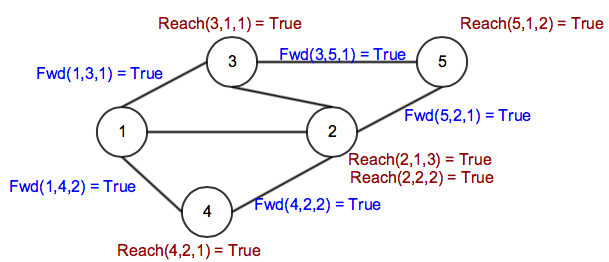
\includegraphics[width=8cm]{topoF.png}
	\caption{Values of the network forwarding model. The red and blue arrows denote the paths taken by packet classes 1 and 2 respectively from source switch 1 to destination switch 2}
	\label{fig:model}
\end{figure}
The network forwarding model is demonstrated by an example in \cref{fig:model}. There are two reachability policies, $r1 : 1 >> [5] >> 2$ with $pc=1$ and $r2 : 1 >> 2$ with $pc=2$ and $r1$ is isolated to $r2$. Using the value of $Fwd$ function, we can find out paths for each packet class, and the set of forwarding rules. 

\subsection{Reachability Constraints} \label{sec:reach}
For a reachability policy $s >> d$ and packet class $pc$, the constraints added must ensure that the solution model contains a path from source from destination. One of the constraints required for this is that there must exist a forwarding rule at source to one of its neighbours, and these constraints act as the base case relating the $Fwd$ and $Reach$ functions. 
\begin{equation} \label{eq:src}
	\exists n \in N(s). Fwd(s, n, pc) \wedge Reach(n, pc, 1)
\end{equation}
$Reach(s.pc,0)$ is taken to be $True$. We need a path to destination, thus destination switch must be reachable for some path length : 
\begin{equation} \label{eq:dst}
	\exists k. Reach(dst, pc, k)
\end{equation}
Also, since the destination is supposed to be the last switch in the path, we need to ensure that the destination does not have forwarding rules further : 
\begin{equation}
	\forall n \in N(dst). \ \neg Fwd(dst, n, pc)
\end{equation}
For the solver to find a path, we need inductive constraints propagating reachability backward from destination to source. If a node $n_1$ is reachable in $k$, there must a node $n_2$ which is reachable in  $k-1$ steps and there exists a forwarding rule $n_2 \rightarrow n_1$.
\begin{multline} \label{eq:bckprop}
\forall n_1,k.  Reach(n_1,pc,k) \implies \exists n_2.  n_2 \in N(n_1) \wedge \\ Reach(n_2,pc,k-1) \wedge Fwd(n_2,n_1,pc)
\end{multline} 
The backward propagation is responsible for ensuring there is a topologically valid path from source to destination by using the unit clauses in \cref{eq:dst}, and finding a path from destination back to a switch $sw$ which is a neighbour of $src$. thus $Reach(sw,pc,1)$ would be true from \cref{eq:src} and the reachability policy would be satisfied. 

The above mentioned constraints are sufficient to ensure there is a path from $src$ to $dst$ for packet class $pc$ in terms of the forwarding function $Fwd$. However, since there is no restriction on number of $Fwd$ values that can be true at a switch, we can get multiple forwarding rules at switches, and also multiple paths to the destination. Also, there can exist forwarding loops as well. Howvever, for a reachability policy, we merely require to find a path from $src$ to $dst$, so we can just extract a path from the model by performing a breadth-first search on the model-graph from source to destination. A directed edge exists in the model-graph : $n_1 \rightarrow n_2$ if there is forwarding rule indicated by the model $Fwd(n_1,n_2, pc) = True$. Thus, we extract the relevant rules of the shortest path from source to destination from the model, and the additional rules obtained in the solution (extra paths, forwarding loops) are ignored.  
\subsection{Waypoint Constraints} 
For a reachability policy with waypoints $s >> W >> d$ and packet class $pc$, we add all the constraints specified in \cref{sec:reach} to ensure the existence of a path from source to destination. To satisfy waypoint policies, we need to add constraints so that all $w \in W$ is reachable. 
\begin{equation} \label{eq:waypoints}
	\forall w \in W. \exists k. Reach(w, pc, k)
\end{equation}
However, just ensuring reachability of waypoints is not sufficient. Since, we do not have any restrictions on the count of forwarding rules for a packet class at a switch, it is possible that waypoints are reachable from the source through separate paths, and do not lie in the path from source to destination. Thus, to ensure that all waypoints are reachable in the path from source to destination, we need to add constraints on the count of forwarding rules at each switch. 

Forwarding rule constraints are to ensure that the forwarding function $Fwd$ at a switch forwards to a \emph{single} node which is a \emph{neighbour} or to no node at all (Switches which are not reached in the path and the destination will not have any forwarding rules). We define the forwarding set $FwdSet$ as follows:
\begin{equation}
	FwdSet(sw,pc) = \{n \ | \ Fwd(sw,n,pc)\}
\end{equation}
The $|A|$ function is used to the denote the size of set $A$. The constraint on the forwarding set are that the size of each set must not exceed 1 (0 or 1). The forwarding set constraint is as follows : 
\begin{equation}
		\forall sw,pc . \ |FwdSet(sw,pc)| \leq 1 \label{eq:fwdset}
\end{equation}
The forwarding set constraints ensure that the forwarding rules exist only on the path from source to destination, and no other rules exist in the solution. If a switch has a forwarding rule elsewhere, then it would not have a rule for the path, and the destination will not be reachable. These restrictions will also ensure there are no forwarding loops in the path. 
Since, there is only one path in the model from source and destination, and \cref{eq:waypoints} ensures that waypoints are reachable, therefore, the path from source to destination must traverse through all the waypoints. Since \cref{eq:waypoints} imposes no order on waypoint traversal, the solution will traverse the waypoints in no particular order. 

\subsection{Isolation Constraints}
For a traffic isolation policy $pc_1 || \ pc_2$ means that the paths do not share an link in the same direction in their paths, therefore, at every switch, the forwarding rules for $pc_1$ and $pc_2$ must not forward it to the same switch.  
\begin{equation}
	\forall n_1. \neg ( \exists n_2. Fwd(n_1,n_2,pc_1) \wedge Fwd(n_1,n_2,pc_2)) \label{eq:isolation}
\end{equation}
These constraints are sufficient to ensure that the packet classes $pc_1$ and $pc_2$ would be isolated. 

The isolation constraints is intuitive when coupled with the forwarding set constraints (\cref{eq:fwdset}) as the model only has forwarding rules for the path from source to destination. However, for a reachability policy, we argue that the forwarding set constraints are not required when coupled with the isolation constraints. The reasoning behind this is that the solver would simply remove the extra forwarding rules of a packet class in the model which conflict with the other packet class, as there are no constraints which require the need of these extra forwarding rules for correctness, but are just one solution model in the space of solutions. 

For a security isolation policy, $pc_1$ and $pc_2$ must not share links at all. \cref{eq:isolation} constraint can be modified to enforce bidirectional isolation :
\begin{multline}
\forall n_1. \neg ( \exists n_2. Fwd(n_1,n_2,pc_1) \wedge \\ (Fwd(n_1,n_2,pc_2) \vee Fwd(n_2,n_1,pc_2)) \label{eq:secisolation}
\end{multline}

\subsection{Maintenance Constraints}
For a link maintanence policy of link $sw_1 \rightarrow sw_2$, we need to ensure that for all packet classes, the variable $Fwd(sw_1, sw_2, pc)$ is $False$, otherwise there would be a forwarding rule $sw_1 \rightarrow sw_2$ for $pc$ on the link. Thus, to perform link maintenance, the constraints required are: 
\begin{equation}
	\forall pc. \ \neg Fwd(sw_1, sw_2, pc)
\end{equation}
Similarly, for a switch maintanence policy of switch $sw$, we need to ensure no packet class reaches $sw$, and thus, no path would contain the switch $sw$, and can be removed for maintenance. The constraints required for switch maintenance are as follows : 
\begin{equation}
	\forall pc, k. \ \neg Reach(sw, pc, k)  
\end{equation}

\subsection{Capacity Constraints}
%\subsubsection{Link Capacity Constraints} \label{sec:linkcap}
For a link capacity policy on the link $sw_1 \rightarrow sw_2$ with capacity $\omega$, we use the theory of integer linear arithmetic to add constraints on the link so that capacity used by the flows traversing the link does not exceed $\omega$. In terms of our model, the link capacity policy translates to constraints to ensure that the the occurences of $Fwd(sw_1, sw_2, pc) = True$ for $pc \in PC$ conforms to the capacity specified in the policy, as the forwarding rule $sw1 \rightarrow sw2$ means that the link is being used by the particular packet class.
 
Let $C(sw_1,sw_2,pc)$ be the cumulative capacity function of the link used by all packet classes less than equal to $pc$. Since we use integers for denoting the packet class, and thus, we have total order of the set of packet classes. We use this to create inductive constraints to sum over the set of Boolean variables $Fwd(sw_1, sw_2,pc)$. Let $PC : [0, \lambda]$ be the set of packet classes and the $W(pc)$ is the capacity of packet class $pc$ ($W$ can be uniform or non-uniform for all packet classes). 
The base case constraint for the capacity function is for $pc = 0$ (the minimum element of $PC$) :
\begin{equation}
	Fwd(sw_1, sw_2, 0) \implies C(sw_1, sw_2, 0) == W(0)
\end{equation}
\begin{equation}
	\neg Fwd(sw_1, sw_2, 0) \implies C(sw_1, sw_2, 0) == 0
\end{equation} 
The inductive constraints for the capacity function are as follows if link is used : 
\begin{multline}
	\forall pc > 0. Fwd(sw_1,sw_2,pc) \implies \\ C(sw_1, sw_2, pc) ==  C(sw_1. sw_2, pc - 1) + W(pc)
\end{multline}
If the link is not used, the constraints are as follows : 
\begin{multline}
\forall pc > 0. \neg Fwd(sw_1,sw_2,pc) \implies \\ C(sw_1, sw_2, pc) ==  C(sw_1. sw_2, pc - 1)
\end{multline}
If $pc$ uses the link $sw_1 \rightarrow sw_2$, we add $W(pc)$ to $C(sw_1,$ $sw_2,pc-1)$, or add 0 to it if link is not being used. Thus, we define the cumulative capacity constraints using inductive constraints. To satisfy the capacity policy, the total capacity used should not exceed input $\omega$. $\lambda$ is the greatest element in the set $PC$. 
\begin{equation}
	C(sw_1, sw_2, \lambda) \leq \omega	
\end{equation} 

\section{Constraint Evaluation}
In the section, we evaluate the number of constraints required to add to the z3 Solver. Let $|S|$ be the number of switches in the topology, $|L|$ be the number of edges in the topology, $|PC|$ be the number of packet classes, $|I|$ be the number of traffic isolation policies and $\mu$ be the max path length. Let $deg$ be the maximum number of neighbours for a switch (degree of the topology).

We encode the forwarding set constraint (\cref{eq:fwdset}) using a SAT encoding rather than an SMT encoding for better performance. To express the constraint that the count of forwarding rules is not more than one, we can do this by adding an $or$ of clauses, where each clause is an $and$ of one rule set to true and all others set to false. An example for switch s and neighbours \{t,u\} is \newline
\verb|(or| \\
\hspace*{10pt}\verb|(and Fwd(s, t, pc)|  \verb|(not Fwd(s, u, pc)))| \\
\hspace*{10pt}\verb|(and Fwd(s, u, pc)|  \verb|(not Fwd(s, t, pc)))| \\
\hspace*{10pt}\verb|(and (not Fwd(s, u, pc))|  \verb|(not Fwd(s, t, pc)))|\\
\verb|)| 

Thus, the number of terms in a forwarding rule constraint for a switch and packet class is $deg \times (deg+1)$. We add a single \verb|or| constraint for each switch and packet class in the network. Therefore, the count of constraints is $|S| \times |PC|$.

The major bulk of time is consumed by the creation of the constraints for backward propagation of reachability (\cref{eq:bckprop}). The number of constraints added to the solver is $|S| \times |PC| \times \mu$. We are using a quantifier-free encoding for better performance, so expressing the $exists$ is done by a $or$ clause of the set of neighbours for a switch. Therefore, the size of each constraint is $deg$. 

For each traffic isolation policy, we need to add constraints for each edge of the network, so that the two packet classes dont share the edge. Therefore, the number of constraints added is $|L| \times |I|$ and the size of each constraint is constant size of two terms.

\begin{table}[H]
\begin{center}
	\begin{tabular}{||m{6em} | m{7em} | m{7em} ||} 
		\hline
		Constraints & Number & Size \\ [0.5ex] 
		\hline\hline
		Forwarding Rules & $|S| \times |PC| $ & $deg \times (deg + 1)$ \\ [0.5ex] 
		\hline
		Reachability Propagations & $|S| \times |PC| \times \mu $ & $deg$ \\ [0.5ex] 
		\hline
		Isolation & $|L| \times |I|$ & 2 \\
		\hline
	\end{tabular}
\end{center}
\caption{Number and Size of Constraints} \label{tab:title} 
\end{table}

\section{Tactics} \label{sec:tactic}
If we consider reachability between two end-switches, the synthesis problem translates to choosing a path from the solution space of all paths from the source to destination such that the chosen path satisfies all policies like waypoints and isolation. Datacenter topologies have multiple paths between endpoints to provide full bisection bandwidth. This feature of datacenters ensues that the solution space of paths for a pair of endpoints is large. 

For example, consider the fat-tree topology in \cref{fattree}. The number of paths under length 10 between two edge  switches in the same pod is 242 and two edge switches in different pods is 272. If we consider the synthesis of $n$ reachability policies, the problem roughly translates to finding a solution in the solution space of size $n \times 242$ which satisfies all policies. 
\begin{figure}[H]
	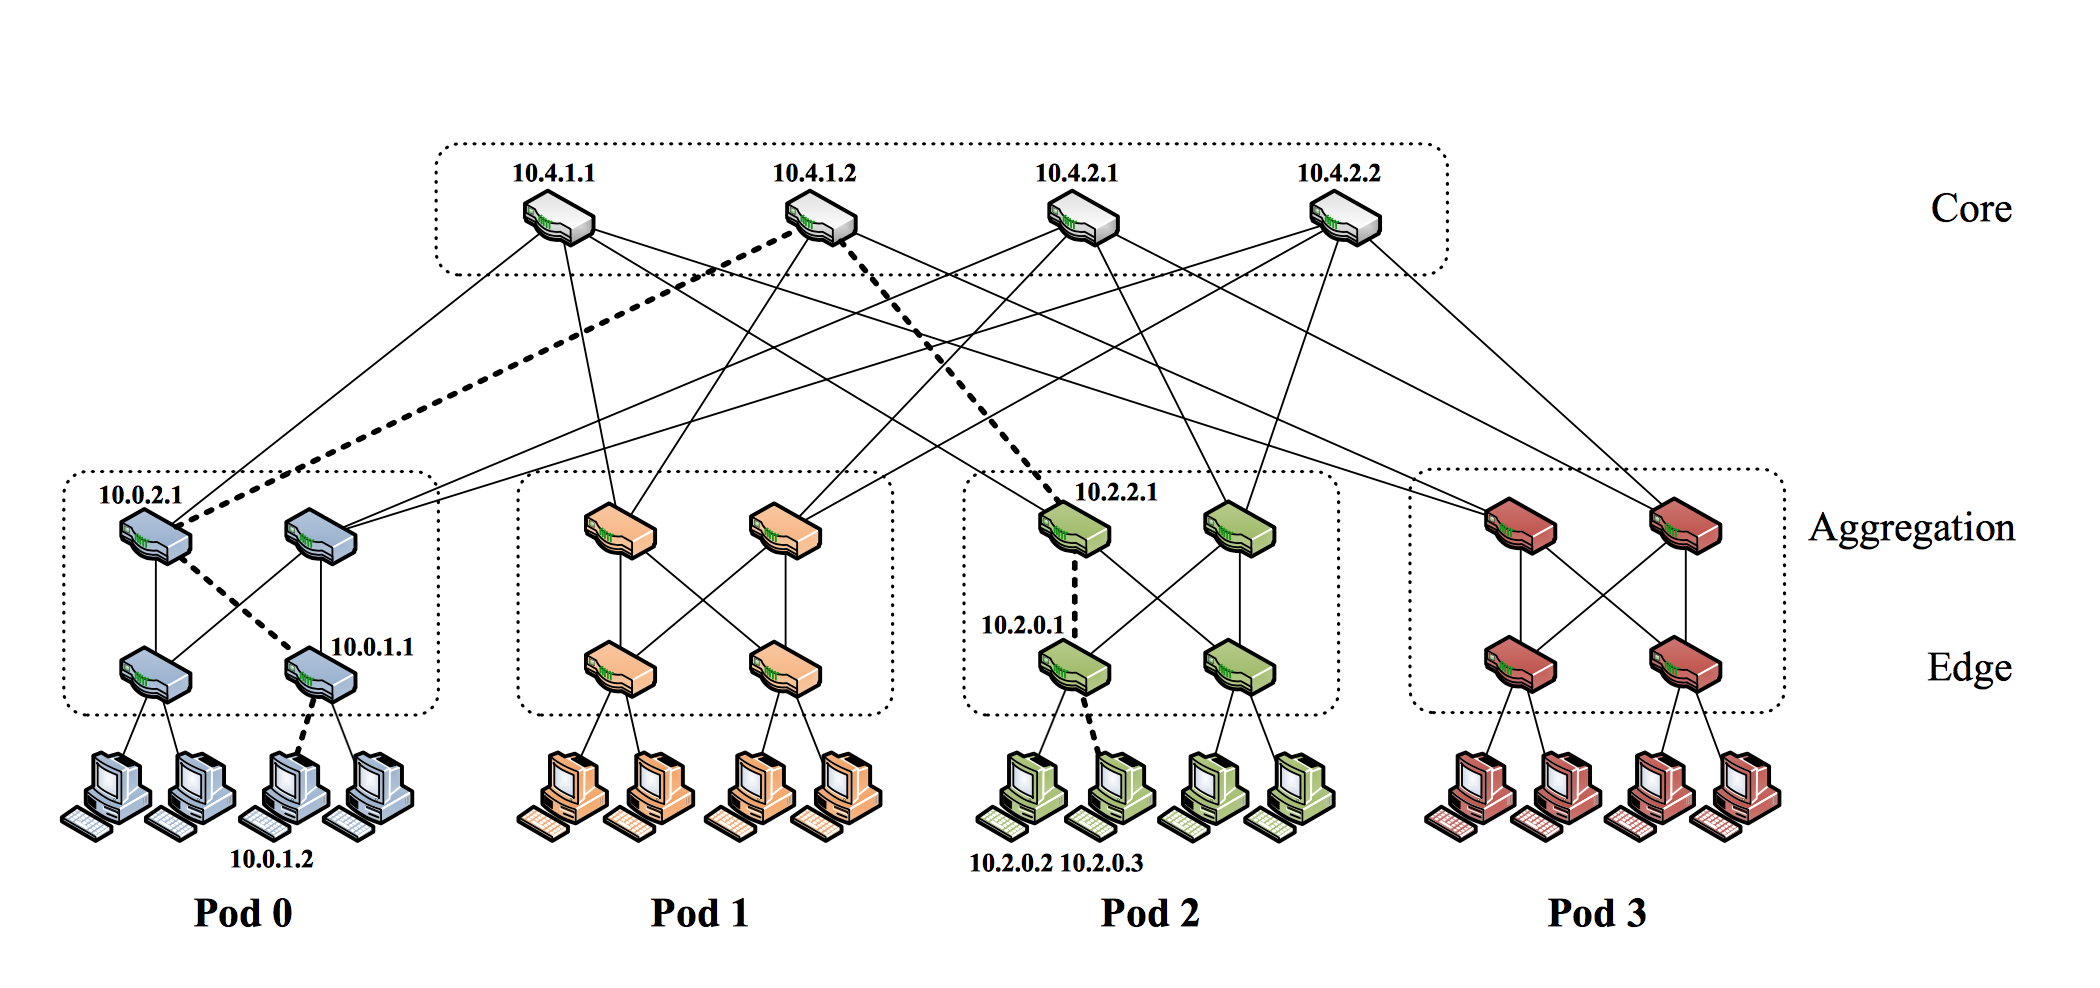
\includegraphics[width=8cm]{fattree.png}
	\caption{Fat Tree Topology}
	\label{fattree}
\end{figure}
We can leverage the network structure of specific topologies to reduce the solution space. In the case of \cref{fattree}, the 272 paths between two edge switches would contain many paths which can be avoided, like paths which traverse through edge switches other than the source/destination, or paths which would be  going from the aggregate to core and back multiple times. 

Tactics are abstractions to impose a high-level restriction on the paths by leveraging the network structure. An example tactic for the fat-tree topology would be that a path connecting two edge switches must not traverse through another edge switch (unless we have a edge switch which is a waypoint). The advantage of tactics is that we would like to provide an expressive framework for operators to provide some insights on the properties of the path without drastically reducing the solution space of paths. 

%Let us define $Lb$ be the set of labels and $S$ be the set of switches in the topology. Let $\phi : S \rightarrow Lb$ be the labelling function and maps switches to a label in $Lb$. One example for $\phi$ in the fat-tree topology in \cref{fattree} can be that we map all switches in the same level(core, aggregate or edge) to the same level, leveraging the hierarchical structure.
%\begin{mydef}
%	A tactic $T$ is a regular expression over the alphabel $Lb$. We construct an associated automaton $A^T$ which is the automaton of the regular expression with every state accepting except the sink state (non-final state with a self-loop over all alphabets).
%\end{mydef}
%A path $P$ is a word over the alphabet $S$. Let $\Phi : S^* \rightarrow Lb^*$ be the path-labelling function which maps each switch in the word to its corresponding label.  
%\begin{equation}
%	P \models T \iff  \Phi(P) \in L(A^T) 
%\end{equation}
%where $L(A^T)$ is the language of automaton $A^T$. The rationale behind the associated automaton $A^T$ is that the automaton accepts prefixes of the label-path, and rejects prefixes which cannot lead to a path satisfying the regular expression of the tactic (by reaching a sink state). 
%
%We demonstrate the example of a tactic with the fat-tree topology in \cref{fattree}. Let $Lb = \{c, a, e\}$. The labelling function $\phi$ maps each core switch to $c$, each aggregate switch to $a$ and every edge switch to $e$. For a path connecting two edge switches, let us define $T_e$ as $(e .^* e) \wedge \neg (e .^* e .^* e)$. This tactic says that the path connecting the two edge switches must not traverse through a edge switch.

\subsection{Synthesis with Tactics}
The tactic defined in the earlier section is a general framework of specify path properties based on network structure. However, adding constraints to ensure the path satisfies the tactic is \emph{slower} than without using tactics. In our synthesis algorithm, the backward reachability propagation constraints are the most significant in terms of time taken and complexity. 
\begin{multline}
\forall n_1,k.  Reach(n_1,pc,k) \implies \exists n_2.  n_2 \in N(n_1) \wedge \\ Reach(n_2,pc,k-1) \wedge Fwd(n_2,n_1,pc)
\end{multline} 
To prune these type of constraints, the question we need to answer is this: If switch $n_1$ with label $\phi(n_1)$ exists in a word at position $k$, what labels can exist in the word at position $k - 1$ such that the word does not reach a sink state in the tactic automaton. By eliminating words which lead the automaton to the sink state, we eliminate the paths which will not satisfy the tactic. For example, the tactic $T_e$ : $(e .^* e) \wedge \neg (e .^* e .^* e)$ which specifies that the path must start and end at a edge switch, and traverse through other edge switches. For $k > 2$ and label $a$, we can observe that the label preceeding it cannot be $e$ if the automaton is not in a sink state (since label $e$ does not come up in the word except the first and the last character). Thus, while adding constraints for a switch of label $a$ and $k > 2$, we can remove neighbours which have label $e$.  

Let us formalise this notion of finding local label patterns based on a tactic $T$ and associated automaton $A^T$ over the alphabet $Lb$. Let $w[k+1]$ denotes the $(k + 1)^{th}$ character of the word. The automaton $A^T$ will accept all words except those which lead it to the sink state. We use the automaton to construct a set of reachable paths for switch label $lb$ and path length $k$. 
\begin{mydef}
	$\Gamma(lb, k)$ is the set of reachable paths such that for each $w \in \Gamma(lb, k)$: 
	\begin{enumerate}
		\item $w \in L(A^T)$
		\item $w \in Lb^{k+1}$
		\item $w[k+1] = lb$
		\item $w$ is a valid label-path in the topology
	\end{enumerate}
\end{mydef}
The first and second requirement is to reason about the backward reachability propagation constraints \newline $Reach(sw, pc, k)$ for switches $sw \in S$ for which $\phi(sw) = lb$. The input to the automaton $A^T$ is restricted based on the topology and label-mapping, and the third requirement is to prune the words to valid label-paths of the topology. In our running example of the fat-tree topology, we can see that neighbours of core switches($c$) are only aggregate switches($a$). Therefore, in a valid label-path, after reading a $c$, we can only read the character $a$. We create a label adjacency matrix of the topology and prune the words in $\Gamma$. 
\begin{mydef} 
	$\Delta(lb, k)$ is the set of labels such that for each $l \in \Delta(lb, k) \iff \exists w \in \Gamma(lb, k).  w[k] = l$ 
\end{mydef}
where $w[k]$ denotes the $k^{th}$ character in the word. 

After computing $\Delta(lb, k)$, we can modify the backward reachability propagation constraints to include neighbours whose labels are in  $\Delta(lb, k)$. 
\begin{multline}
\forall n_1,k.  Reach(n_1,pc,k) \implies \exists n_2.  n_2 \in N(n_1) \wedge \\ \phi(n_2) \in 
\Delta(\phi(n_1), k) \wedge Reach(n_2,pc,k-1) \\ \wedge Fwd(n_2,n_1,pc)
\end{multline} 
If $\Delta(lb, k) = \emptyset$, then $Reach(sw, pc, k) = False$ for switches $sw \in S$ for which $\phi(sw) = lb$. 

To find the $\Delta$s for a tactic, we use a dynamic programming approach of finding all valid label words of length $k$ accepted by the associated automaton ($\forall lb$. $\Gamma(lb, k)$) by using the valid label words of length $k-1$ (we also store the last state the automaton is in), and make one valid transition on labels (validity is based on two factors : automaton doesn't reach the sink state, and the current label and previous label are connected in the topology). After computing the $\Gamma$s, we can compute $\Delta(lb,k)$ by examining $\Gamma(lb,k)$ to find labels at the $k^{th}$ position.
\begin{figure}[h!]
	\centering
	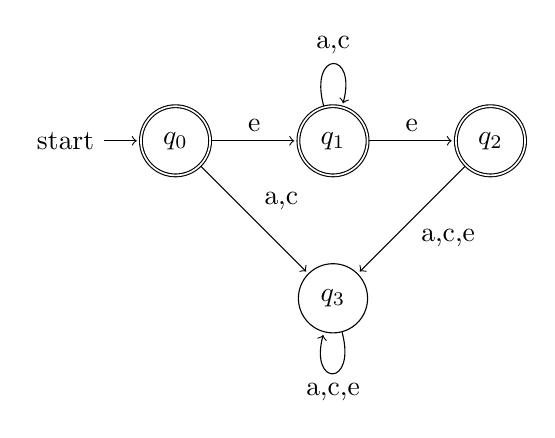
\begin{tikzpicture}[shorten >=1pt,node distance=2cm,on grid,auto] 
	\node[state,accepting, initial] (q_0)   {$q_0$}; 
	\node[state, accepting] (q_1) [right=of q_0] {$q_1$}; 
	\node[state,accepting] (q_2) [right=of q_1] {$q_2$}; 
	\node[state] (q_3) [below=of q_1] {$q_3$}; 
	\path[->] 
	(q_0) edge  node {e} (q_1)
	edge node {a,c} (q_3)
	(q_1) edge  node  {e} (q_2)
	edge [loop above] node {a,c} ()
	(q_2) edge node {a,c,e} (q_3)
	(q_3) edge [loop below] node {a,c,e} ();
	\end{tikzpicture}
	\caption{Associated automaton $A^T$ for tactic $T_e$}
	\label{fig:tactice}
\end{figure}

We demonstrate the advantages of tactics with an example. Consider the tactic $T_e : (e .^* e) \wedge \neg (e .^* e .^* e)$ and its associated automaton(\cref{fig:tactice}). 
\[
\Gamma(a, 2) = \emptyset, \  \Gamma(e, 2) = \{eae\}, \ \Gamma(c, 2) = \{eac\} 
\] 
\[
\Delta(a, 2) = \emptyset, \ \Delta(e,2) = \{a\}, \ \Delta(c,2) = \{a\}
\]
Thus, $\forall sw,pc. \ \phi(sw) = a \ \wedge \ \Delta(a, 2) = \emptyset \implies \\ Reach(sw,pc,2) = False$ and we do not add backward reachability propagation constraints for the term $Reach(sw,pc,2)$. 
% If we did not have the restriction of topologically valid label-paths in $\Gamma$, then $\Gamma(a, 2) =  \{eaa, eca\}$, resulting in $\Delta(a,2) = \{a,c\}$. 

Incorporating tactics in the synthesis is sound. If the tactic imposes an restriction to the path other than the source and destination, then the procedure is incomplete. However, tactics can be used to specify restrictions which would be reasonably complete, thus speeding up the synthesis. Even though we have defined a general framework to specify tactics using regular expressions, since the synthesis constraints depend on local behaviours, not every tactic would provide a speedup. For example the tactic $\neg (.^* c a c a c .^*)$ which specifies that a path must not traverse through the core switch layer more than twice, will not provide  speedup, bacause we cannot deduce any local patterns from the associated automaton as the regular expression is trying to count the number of times the path traverses a core switch, and thus it cannot remove any label from its preceding set as count is a global pattern and our approach can only use local patterns to speedup synthesis.  

\section{Network Surgery}
Network surgery is the technique of performing equivalent network transformations to eliminate redudant constraints required for synthesis of switch rules. One of the properties of the path found by the synthesis solver is that it is simple (i.e no loops). Using this property, we can create slices of the topology where a packet class' path will reside completely, thus not requiring to add constraints for switches in other slices of the topology. 

To create the topology slices, we use Schmidt's linear-time algorithm\cite{schmidt} to find bridges in the graph. A bridge is an edge in the topology, which when removed, partitions the graph into two disconnected components. <write-about-slices>. 

Consider a reachability policy where the source and destination switches belong to the same topology slice. Since, the bridge edge is the only edge connected vertices of this slice with the rest of the graph, the path for the reachability policy will be contained in the topology slice and not cross the bridge (otherwise the path would have to traverse through the bridge twice back and forth which is not permitted). 

Formally, let us define the slices of the topology as $S_1, S_2, ..., S_n \subset S$. We define the slice neighbour function for the slices as $N_{S_i}(s) = \{v | v \in S_i \wedge (s,v) \in L\}$. If there is a reachability policy $(r, pc)$ with $src,dst \in S_i$, we can replace the switch domain $S$ by $S_i$ and the neighbour function $N$ by $N_{S_i}$ in the constraint formation for reachability. For example, the backward reachability propagation constraints for a policy in slice $S_i$ can be modified to : 
\begin{multline}
\forall n_1,k.  n_1 \in S_i \wedge Reach(n_1,pc,k) \implies \exists n_2. n_2 \in N_{S_i}(n_1) \\ \wedge  Reach(n_2,pc,k-1) \wedge Fwd(n_2,n_1,pc)
\end{multline}
For packet classes isolated with packet class $pc$, only links in $S_i$ are needed to be isolated, as the path will be confined to topology slice $S_i$. 

\section{Optimistic Synthesis} \label{sec:optimistic}

\section{Implementation}

%\section{Multicast Policies} \label{sec:mcast}
%Genesis supports two multicast policies, \emph{normal} and \emph{equal} multicast. Genesis will leverage the Openflow functionality to send a packet to multiple outports to create multicast group paths from source to the destinations. The normal multicast is IP-multicast from a source to a group of destinations without any restrictions. \\
%To aid in achieving approximate synchrony in multicast groups for distributed systems \cite{mcast}, Genesis supports \emph{equal} multicast ensures that paths from the source to each destination in the multicast group to have the same path lengths to minimize the disparity of message latencies to each destination. \\
%
%\subsection{Path Constraints}
%To support multicast, we needed to remove the restriction of next-hop forwarding set on our forwarding model. So, for a multicast packet class, our model can forward it to multiple nodes.  \\
%However, this can cause the possibility of cycles in the graph. The multicast group paths creates a \emph{tree} with the source as root and the leaves are the destination. To remove cycles, we mark nodes in the graph with a rank number, which is the depth of the node in the multicast path tree. We use an \emph{uninterpreted function R} to add constraints for the rank function to ensure acyclicity of the paths.
%\[
%R(src, pc) = 0  \label{ranksrc} \tag{M1}
%\]
%To ensure the nodes further in the path have greater ranks, we add the following constraint. 
%\[
%\forall n_1, n_2.(Fwd(n_1,n_2,pc) \implies R(n_1,pc) < R(n_2,pc))  \label{ranknode} \tag{M2}
%\]
%Since the forwarding model can send packets from a node to multiple next-hop nodes, we need constraints to ensure that two paths do not lead to the same destination. Let us define $recvSet(n,pc)$ as the set of all nodes the node $n$ receives the packet.
%\[
% recvSet(n,pc) = \{n' | Fwd(n',n,pc) = True\}
% \]
%\[
%\forall n. \ |recvSet(n,pc)| \leq 1 \label{ranknode} \tag{M3}
%\] 
%For \emph{equal multicast policy}, all the paths to destinations must have equal path lengths. 
%\[
% \forall d \in dstSet \ \exists k .(Reach(d, pc, k) \wedge \neg Reach(d, pc, k - 1) ) \label{eqmdst} \tag{EM1}
%\]
%However, there are some important \emph{caveats} to the multicast policy enforcement. The above constraints ensure paths to the destinations specified in the policy, but also provides various paths to nodes which are not specified in the policy (still a correct enforcement of the policy). Instead of adding constraints to the model to ensure the model only gives paths to the destinations and no more, we simply extract the paths we require from the model and ignore the extra paths. Another assumption is that we are dealing with multicast policies independently. If we change the system to incorporate inter-policy interactions with mutlicast policy, we will have to include constraints to provide a solution which does not contain paths not required by the policy.
%
%\section{Policy Interactions}
%Consider our input policies, like reachability and waypoint policies. For a packet class, the enforcement of these policies do not require the system to have information of other packet classes, and we can synthesize each of these packet classes independently. Since Z3 is expontential in the number of flows fed to the model, the best approach is to synthesize these packet classes independently. \\
%However, policy interactions complicate this approach. Policy interaction is defined as the event of two packet classes which have to be reasoned together by Genesis to ensure correctness, like traffic isolation policies. Therefore, if $pc_1$ and $pc_2$ have to satisfy a isolation policy, naive Genesis needs to add both the flow constraints to Z3 together and the synthesize the forwarding rules. \\
%We define a \emph{Relational Class} to be the maximal set of packet classes which need to synthesized together in Z3 for correct policy enforcement. For the present case, the only policy interactions are due to isolation policies, so the construction of relational classes for the set of packet classes consider only isolation policies. \\
%The property of an $RC$ is as follows : for each $pc_1$ in the $RC$, there exists a $pc_2$ in the $RC$ such that $pc_1$ and $pc_2$ are isolated and there does not exist a $pc_3$ not in $RC$ such that $pc_1$ and $pc_3$ are isolated. 
%\[
%\forall pc_1. ( pc_1 \in RC \implies \exists pc_2 \in RC.( Isolated(pc_1,pc_2))
%\]
%\[ \wedge \neg (\exists pc_3 \notin RC. (Isolated(pc_1,pc_3)))
%\]
%The algorithm for creating Relational Classes is simple, initially create a $RC$ for each packet class, and for each isolation policy, if the packet classes reside in different $RCs$, merge the two $RCs$ to create a new $RC$.
%
%\subsection{Advantages of Relational Classes}
%The biggest advantage of Relational Classes is the separation of packet classes which need to be input to Z3 together, thus reducing the synthesis complexity to expotential in the largest Relational Class. This in worst case can be the complete packet class set, but we would leverage policy behaviours used in datacenters to evaluate on real-life cases of the size of the largest relational class. \\ \\
%Another advantage of dividing the packet class space is the opportunity to do \emph{parallel} synthesis of each relational class, thus leveraging the powerful hardware available abundantly in recent times. Z3 is a single process, single threaded application which does not leverage parallelism, so we leverage relational classes for parallelism at a higher level.  \\
%
%\section{Network Change Synthesis}
%There are two change events which would require reconfiguration of forwarding rules : change in policies and change in network topology. By leveraging the concept of relational classes, we can perform network change synthesis.
%\begin{itemize}
%	\item \textbf{Policy Change Synthesis} : This would require synthesis of only those relational classes which are being affected by the policy changes (addition of new classes and policies, modification of existing changes). The naive approach is to resynthesize the complete $RCs$, but there could be approaches to leverage the existing model to make incremental changes. 
%	\item \textbf{Topology Change Synthesis} : This would require synthesis of only those relational classes which are being affected by the topology change (link/switch failures). 
%\end{itemize}
%
%\section{Optimistic Synthesis} \label{sec:Optimistic}
%A common thread to the clean-state synthesis model we are working on, and the network change synthesis is an efficient way of synthesizing relational classes. The naive approach of synthesizing the relational class by adding the constraints of all packet classes scales poorly ($300s$ for 100 flows in a 10-clique topology). Isolation policies may not all-to-all (all flows isolated from one other) and we can leverage these policy interactions to synthesize packet classes in a relational class independently, and validating the enforcement of isolation policies. \\
%A \emph{relational class graph} is a graph with the packet classes as vertices of the graph, and the edges model the inter-policy interactions (for our case, isolation policies). We leverage the structure of the RC graph to perform Optimistic synthesis. The key motivation is as follows : Instead of performing the synthesis of the complete RC, split it into partitions, and solve them such that the solution obtained from the individual partitions satisfy all the input policies. 
%\begin{figure}[H] 
%	\includegraphics[width=8cm]{rcGraph.png}
%	\caption{Relational Class Graph and Optimistic Partitions}
%	\label{fig:Optimistic}
%\end{figure}
%Consider the RC graph in \cref{fig:Optimistic}. One of the heuristics that can be used to partition the RC graph is minimising the \emph{cut edges} between the two components (the vertices of the cut edges lie in different components). The rationale behind the heuristic is that since we intend to perform the synthesis of both the components separately, the partition should have the least number of constraints between themselves, thus providing more freedom for the separate solutions to satisfy the complete constraints. The synthesis approach is \emph{Optimistic}, because the smaller solutions may or may not be correct. To improve accuracy, we feed the solution of the first partition to the second partition as constraints (so that the second partition does not produce a  inconsistent solution). \\
%An issue with this approach is that the solution of the first partition may not be satisfiable with the second partition, but the complete RC graph has a solution. A preliminary idea is to add the troublesome packet classes into the first partition and resynthesize. \\
%The Optimistic synthesis procedure can be applied to the RC graph component recursively, and propagating the solutions to the other connected components, with the base case being a component of a minimum size, or the number of cut edges less than a threshold value. The advantages of Optimistic synthesis is that we can achieve linear time complexity for the number of flows.
%
%\subsection{Solution Recovery} \label{sec:recovery}
%The shortcomings of the Optimistic synthesis approach is that the partial solution synthesized on a partition may not be have a complete solution for the entire graph. To achieve swift convergence to a correct solution, we devise various recovery techniques. \\
%The solution recovery approach leverages Z3's functionality of obtaining unsatisfiable cores. We track the assertions corresponding to partial solutions to the solver (Z3 provides this functionality) and if the solver returns \texttt{unsat}, then we extract the unsatisfiable cores which are the partial solutions which cause the unsatisfiability. These solutions are propagated back to their partitions, and the solver will return a solution to these cores which are different from the unsatisfiable cores provided. \\
%The rationale behind tracking the partial solutions is that those are the problematic constraints and can cause the solver to return  \texttt{unsat} even when they exist a solution due to incompatible partial solutions. This recovery leverages the failed partial solutions to find new partial solutions. \\
%For boundedness, we perform the recovery a fixed number of times (not decided on this yet) and for each increasing recovery, the unsatisfiable partial solutions are accumulated, and the solver has to find a partial solution which is different from all previous falied solutions. \\
%For example in \cref{fig:Optimistic}, the solution of PC1 will be propagated as a constraint to the partition $\{PC2,PC5, PC0\}$. If the solver returns \texttt{unsat}, for recovery and $PC1$ as the unsatisfiable core, we resynthesize partition $\{PC1, PC3$, $PC4\}$ with the additional constraint that the solution obtained for $PC1$ is different from the earlier solution of $PC1$. We repeat this a finite amount of times till we succeed or return failure for this recovery approach. 
%
%\subsection{Incremental Recovery}
%The correct procedure to solve the synthesis is to add constraints for every flow to the z3 solver and check for satisfiability. Since, this is order of expotential in the number of flows in a relational graph, we try to speed up by using a Optimistic synthesis approach. The problem of fuzzy synthesis is that the partial solutions are evaluated on parts of the complete graph, thus, there is no guarantees of finding a solution. The success of finding a correct partial situation will increase with the size of the graph on which z3 finds a partial solution.
%\\
% 
% Thus, another recovery approach we use with fuzzy synthesis is incrementing the size of the base graph on which z3 operates if fuzzy synthesis with solution recovery cannot provide a solution with a smaller base graph size on which z3 finds the partial solution. This recovery method doubles the graph size each failure, till we reach the size of topology, which translates to a normal synthesis approach. Thus, the fuzzy synthesis approach with solution and incremental recovery will produce a correct solution, if one exists. The best case complexity is better than expotential, while the worst case complexity is expotential. 
%
%\section{GPL : Genesis Policy Language} \label{sec:gpl}
%%\subsection{Grammar}
%%\noindent Below is the grammar of GPL (Genesis Policy Language) which can be used to specify the policies to the Genesis synthesiser to obtain the paths for each of the policies. 
%%The non-terminal $D$ is used to generate declaration statements. Since GPL has a restricted syntax, we can infer the types from the right hand value of the declaration statement, so we adopt a Python-like syntax for variables which don't require type declarations. \\
%%The non-terminal $REACH$ is used to specify reachability policies, which is of the form \lstinline{R -> endpoint >> endpoint}. The $>>$ is the reach operator, the first operand specifies the source and the second operand specifies the destination. The non-terminal $endpoint$ is used to specify the IP subnet/address and the next-hop switch connected to the IP subnet/address(\lstinline{endpoint -> ip:sw}). Each reachability policy creates a new packet class. \\
%%The non-terminal $WAYPOINT$ is used to specify reachability policies with waypoints. The operand between the two $>>$ operators specify the list of waypoints the packet class must traverse to. \\
%%The non-terminal $I$ is used to specify traffic isolation policies. The isolate operator $||$ is used to specify isolation policy between two packet classes. \\
%
%\subsection{Interpreter}
%The Genesis interpreter is built using the PLY library (Python-Lex-Yacc) \cite{ply} which parses the input GPL file and add the policies to the Genesis Synthesiser (which has a Policy Database to store the policies). After successful parsing, the Genesis Synthesiser enforces the policies using the normal or fuzzy synthesis approach to find the paths to be followed by each packet class. Following is an example policy file.
%\begin{lstlisting}
%# GPL Reachability Policy Descriptions
%f1 := ip.src=10.0.0.4 : 
%e3 >> [a26] >> e17
%f2 := tcp.port= 80 : e1 >> e12
%f3 := tcp.port= 70 : e1 >> e10
%f4 := ip.src=10.0.0.2 : 
%e1 >> [c78] >> e11
%==
%# GPL Isolation Policies
%f1 || f4
%|| [f1,f2,f3]
%\end{lstlisting}
 

\section{Evaluation}
\begin{figure*} 
	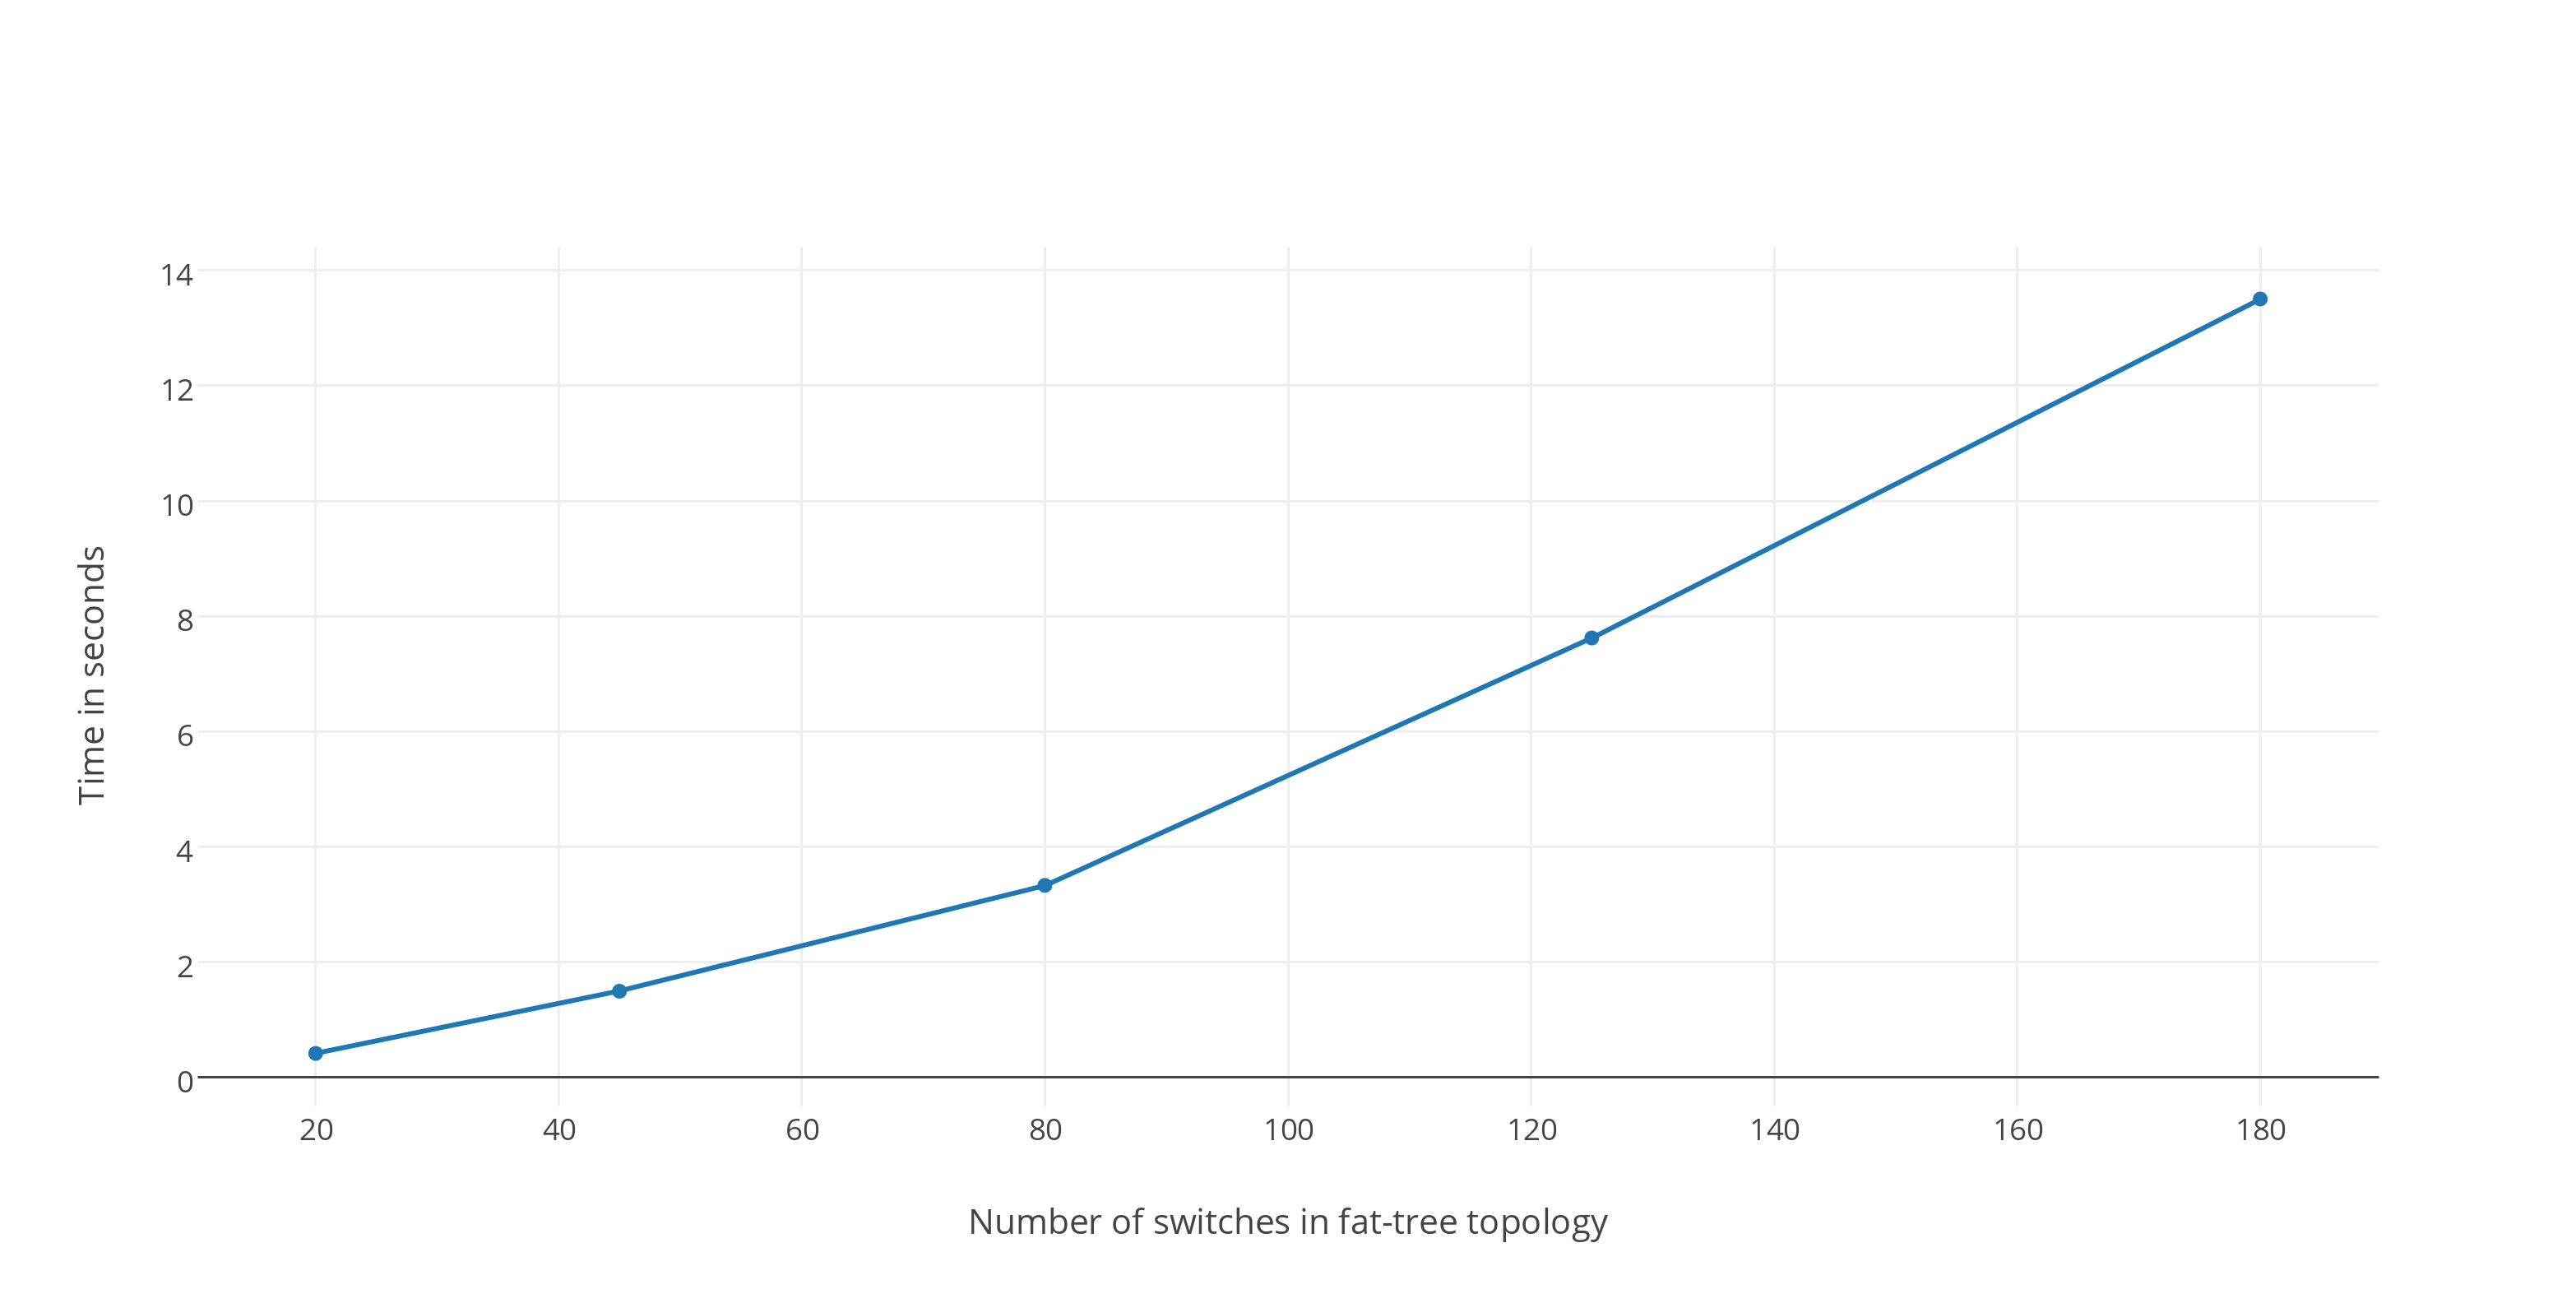
\includegraphics[width=20cm]{GenesisTopo.png}
	\caption{Time taken to synthesize two isolated flows with increasing fat-tree topology sizes}
	\label{fig:topo}
\end{figure*}
\begin{figure*} 
	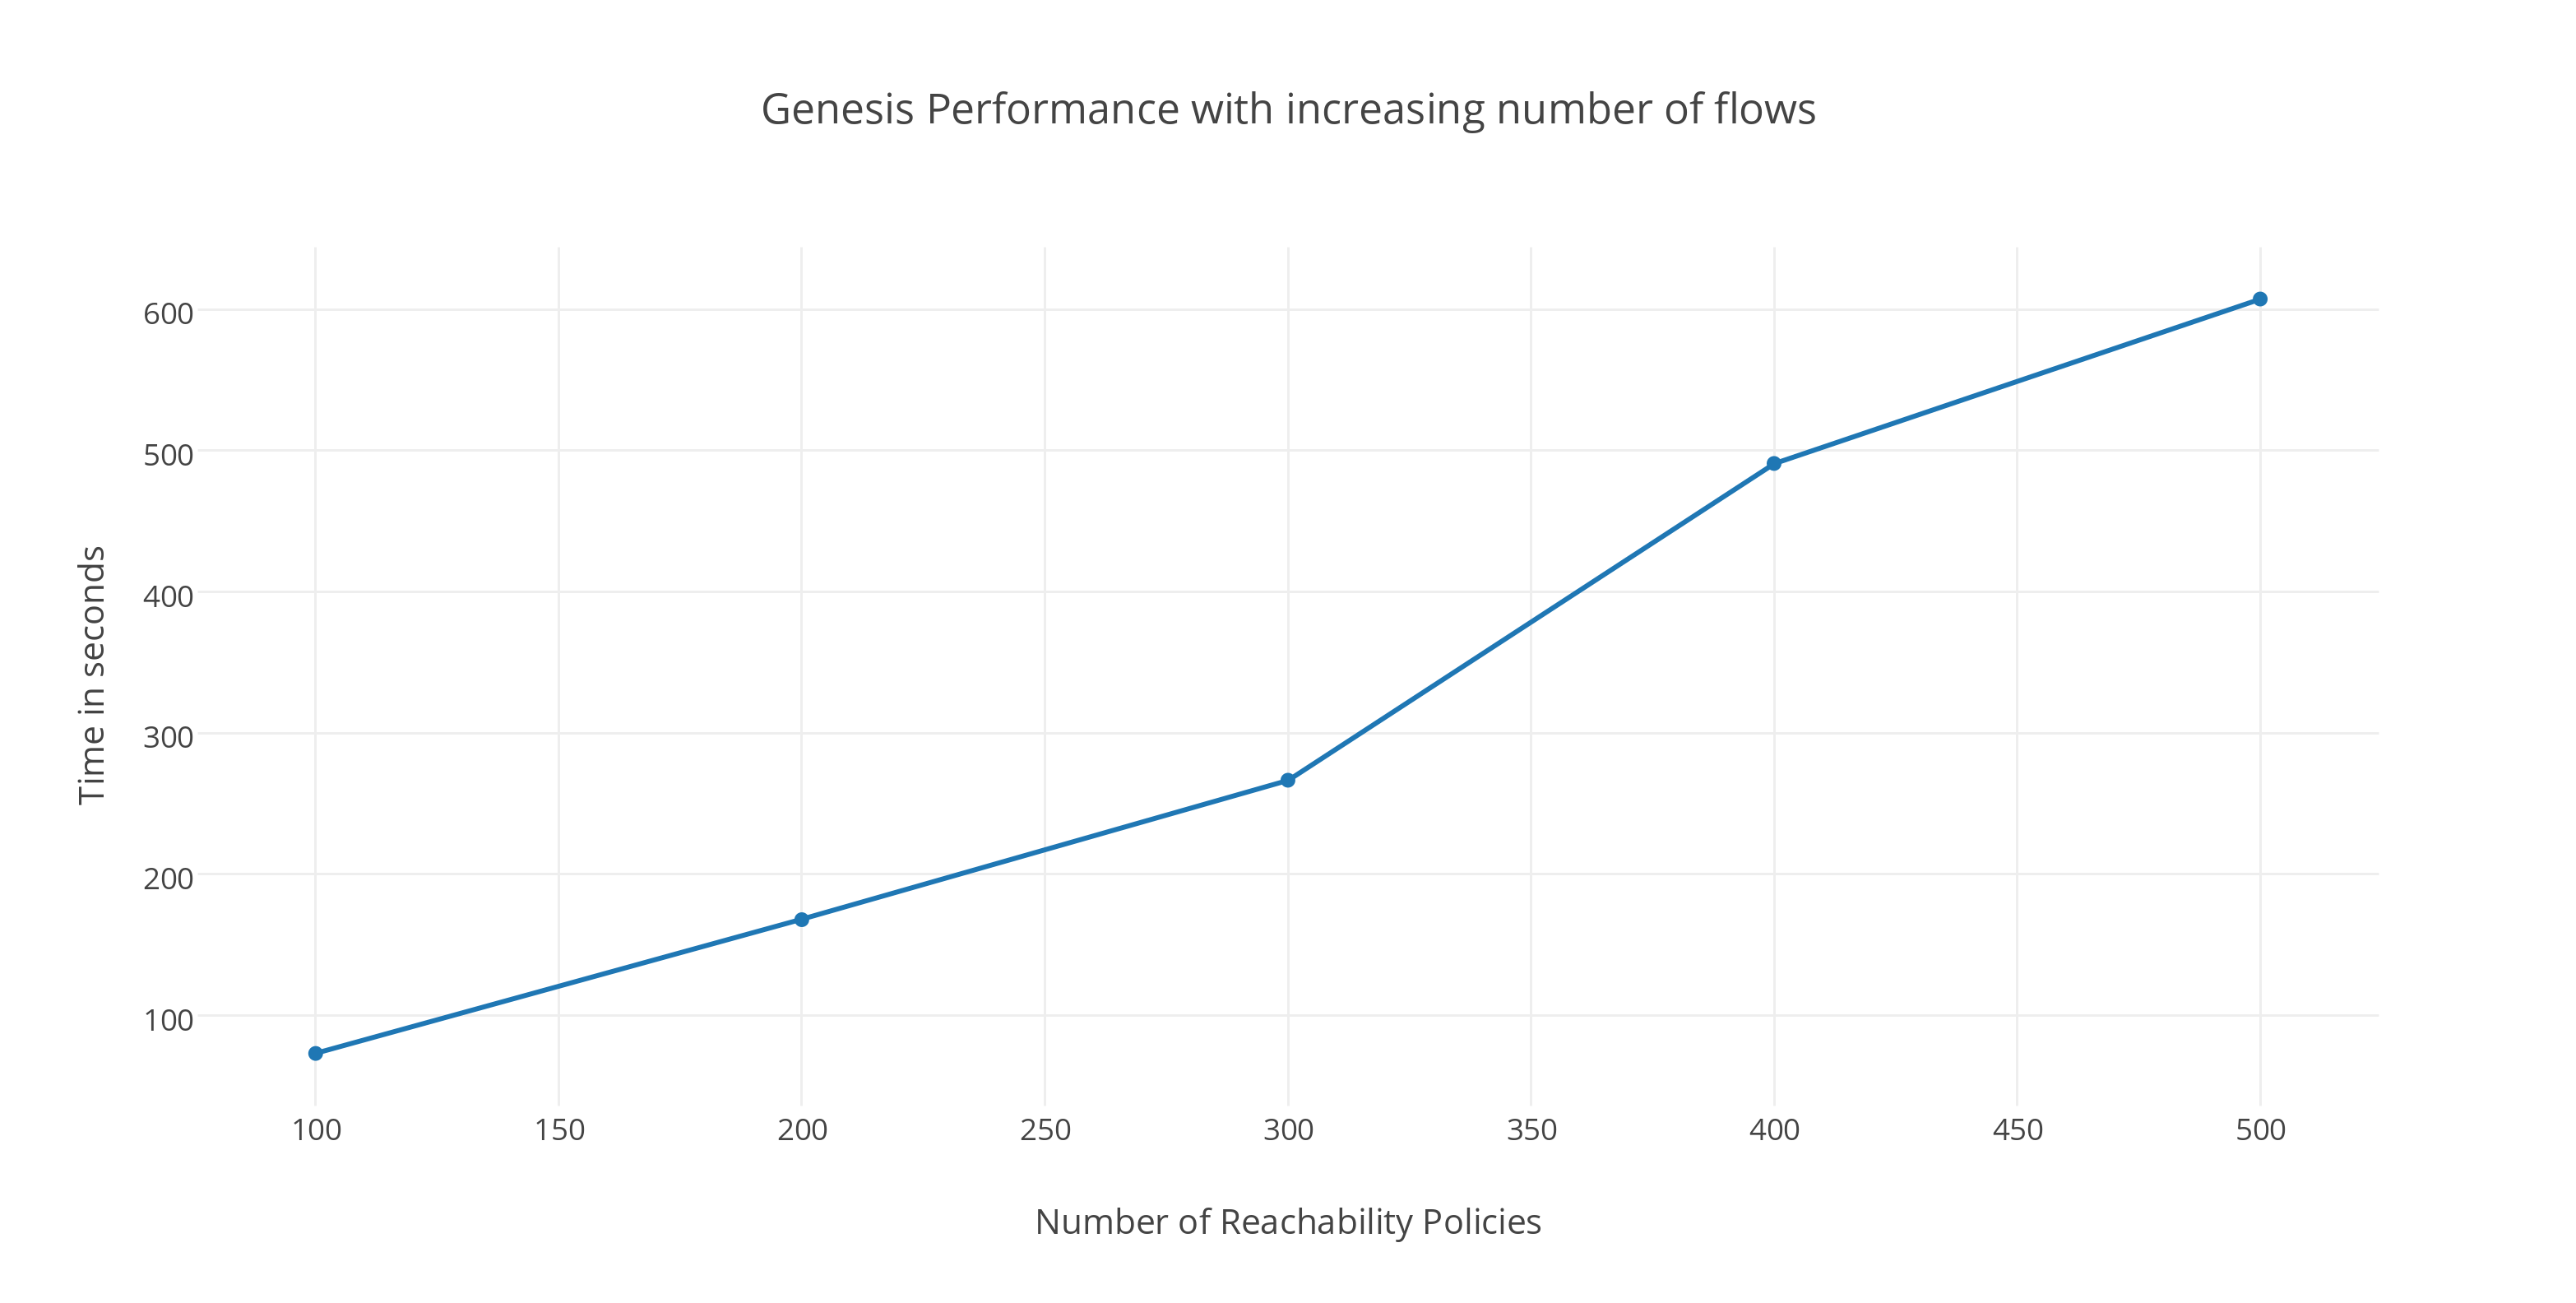
\includegraphics[width=20cm]{GenesisReach.png}
	\caption{Performance plot to synthesis with increasing number of reachability policies in a 45-node fat-tree topology}
	\label{fig:reach}
\end{figure*}
In \cref{fig:topo}, we evaluate the performance of Genesis with respect to increasing topology sizes. We use fat-tree topology, and the policy inputted is two reachability policies where the source and destination are edge switches (one policy has a single aggregate switch as a waypoint). These two policies are isolated to each other. The number of nodes is the X-axis and the Y-axis is the time taken to synthesise the paths for the two input policies. As expected, we can infer a expotential increase with number of switches in the topology. \\
In \cref{fig:reach}, we evaluate the performance of Genesis with respect to increasing number of reachability policies in a 45-node fat-tree topology. The reachability policies have both source and destination as edge switches (without a waypoint) and no isolation between them. The number of policies is the X-axis and the Y-axis is the time taken to synthesise the paths for the two input policies. Though, this problem can be solved simply by DFS, this experiment is more to rationalise the fact the z3 will not have linear complexity for such a case.

\section{Related Work}
\cite{decentralize} tries to synthesize local forwarding rules for a single switch based on a reactive forwarding policy. One of the important considerations for correctness of forwarding rules is that the controller sees all relevant events and rules are not added prematurely. The abstraction for expressing forwarding policies are for individual switches, on the other hand, we try to enforce network-wide policies, so each switch will have different forwarding policy such that the entire network enforces the flow policies. Also, the policies we deal with are proactive, so we need not worry about the controller seeing the relevant events (which is a requirement in synthesizing rules for reactive policies). For all practical purposes, we needn't worry about switch-controller interactions or premature rule installations. \newline
NetEgg \cite{netegg} synthesizes the forwarding policy of a switch using examples of how the switch should function when it receives packets. This deals with the forwarding policy of individual elements, can cannot be used directly to synthesize network-wide policies. \newline
\cite{oneswitch} tries to tackle a similar problem to ours of flow policy enforcement. However their end-point policies are only concerned with reachability (two hosts can talk through specific ingress and egress points). Their rule placement algorithm takes the path of the flow in the network as an input (the routing policy) and place rules on this path to enforce the endpoint policy and taking in consideration switch table constraints. We are trying to tackle the problem without the routing policy as input, as we enforce flow policies which would require different routing policies (like traffic isolation), so we cannot determine the path of the flow beforehand. Our solution can support enforcement of policies which require different routing policies. \cite{distfirewall} builts on the \cite{oneswitch} abstraction to optimize the specific case of distributed firewall policy enforcement using ILP.  \newline
\cite{netgen} NetGen solves the problem of network updates using synthesis. Given a specification which mentions the packet classes, the old path and the new path, NetGen solves the network change problem using a SMT solver. One salient aspect is the use of uninterpreted functions to reduce the number of constraints. 

\section{Conclusion}
\bibliography{references}{}
\bibliographystyle{acm}
 \appendix
 \section{Proofs of NP-hardness} \label{sec:np}
 \subsection{Enforcement of Isolation Policies}
 Given a undirected graph $G=\{V,E\}$ which represents the switch topology denoted in \cref{fig:swtopo} and undirected graph $P =\{R,I\}$ which represents the policy graph. Every vertex $p \in P$ is a reachability policy : $S >> D$ and each edge $i \in I$ which connects vertices $p1$ and $p2$ mean that the paths of $p1$ and $p2$ are isolated from each other. 
 \begin{figure}[H] 
 	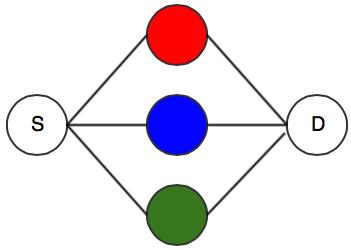
\includegraphics[width=8cm]{color_topo.png}
 	\caption{The switch topology $G$. All circles represent switches and all reachability policies are $S$ to $D$}
 	\label{fig:swtopo}
 \end{figure}
The solution to policy enforcement will be such that each reachability policy $p \in P$ from $S >> D$ will traverse through one of the colored switches $\{red$, $blue$, $green\}$. Color the vertices of $P$ with the switch the path traverses through. If two vertices are connected by an edge in $P$, those flows would be isolated, and thus, will not have the same color. Thus, the problem reduces to finding a 3-graph coloring for $P$, which is NP-complete. Thus, the enforcement of isolation policies is NP-complete. 
 
 In genral, k-coloring (for k > 2) is NP-complete, the policy enforcement problem in a switch topology with k paths from source to destination reduce to a k-coloring problem, and thus is NP-complete. 
 
 \subsection{Enforcement of Waypoint Policies}
 Given a undirected graph $G={V,E}$. Let us assume there exists an polynomial-time algorithm to compute the reachability paths satisfying the policies of the following types on the graph : \\
 \begin{itemize} 
 	\item \textbf{P1} : $v_1 >> v_2 \Rightarrow$ There exists a path from $v_1$ to $v_2$ satisfying all input policies. A property of the path is that it does not have repeat a vertex (no forwarding loops).
 	\item \textbf{P2} : $v_1 >> W >> v_2 \Rightarrow$ The path from $v_1$ to $v_2$  should pass through the vertices in the set $W$ in any order, without repeating a vertex.
 \end{itemize}
 \textbf{Reduction of Hamiltonian Cycle Problem} : Given a undirected graph $G={V,E}$, find $v \in V$ such that the degree of $v$ is the minimum in the graph (Will work for any vertex actually). If a Hamiltonian cycle is present in the graph, it will have the vertex $v$ in the cycle, and one of the edges from $v$.  \\
 Lets take a $n \in Neighbours(v)$. Let the input policies to our algorithm be : 
 \begin{itemize}
 	\item \textbf{P4} : $v >> W >> n$ where $W = V - \{v,n\} $ 
 \end{itemize}
P4 cimputes a simple path from $v$ to $n$ which passes through all the other vertices in the graph which is the Hamiltonian path problem. Since computing the Hamiltonian path is NP-hard, the problem of path computation for the waypoint policies as specified is NP-hard. 
 
\end{document}
